\documentclass{book}

% Fonts and typography

%% Set hypens according to specified language
%\usepackage[utf8]{inputenc}
%\usepackage[italian]{babel}



%% Typography
\usepackage[no-math]{fontspec}
\defaultfontfeatures{Mapping = tex-text, Scale = MatchLowercase}

%% Fonts
\setmainfont[Path=inc/fonts/]{Raleway-Regular.ttf}
\setsansfont[Path=inc/fonts/]{JosefinSans-SemiBold.ttf}
\setmonofont[Path=inc/fonts/]{JosefinSans-Regular.ttf}


%\usepackage{polyglossia}
%\setdefaultlanguage{italian}
%%
% \newfontfamily [ Path = fonts/, ... ] { }
% \setmainfont{Raleway-Regular}
% \setsansfont{JosefinSans-SemiBold}
% \setmonofont [ Path = fonts/, ... ] { }
% \setmonofont[Mapping=tex-ansi]{Menlo}

%% Set Sans font in headings
\usepackage{sectsty}
\allsectionsfont{\sffamily}

%% Set polyglossia language
% \usepackage{polyglossia}
% \setdefaultlanguage[babelshorthands=true]{italian}




% Page

%% Use full page in book style
\usepackage{fullpage}

%% Set line spacing
\usepackage{setspace}
\setstretch{1.625}

%% Disable paragraph indentation
% \usepackage{parskip}

%% Start sections from new page
\let\stdsection\section{}
\renewcommand\section{\newpage\stdsection}


% Colors

\usepackage{xcolor}

%% Tango color scheme
\definecolor{SkyBlue}{HTML}{3465A4}
\definecolor{DarkSkyBlue}{HTML}{204A87}

\definecolor{Plum}{HTML}{75507B}

\definecolor{ScarletRed}{HTML}{CC0000}

\definecolor{Aluminium1}{HTML}{EEEEEC}
\definecolor{Aluminium6}{HTML}{2e3436}

\definecolor{Black}{HTML}{000000}


% Listings

\usepackage{listings}

\lstdefinelanguage{JavaScript}{
  keywords = {typeof, new, true, false, catch, function, return, null, catch, switch, var, if, in, while, do, else, case, break},
  keywordstyle = \color{SkyBlue}\bfseries,
  ndkeywords = {class, export, boolean, throw, implements, import, this},
  ndkeywordstyle = \color{Aluminium6}\bfseries,
  identifierstyle = \color{Black},
  sensitive = false,
  comment = [l]{//},
  morecomment = [s]{/*}{*/},
  commentstyle = \color{Plum}\ttfamily,
  stringstyle = \color{ScarletRed}\ttfamily,
  morestring = [b]',
  morestring = [b]" % chktex 18 [suppress warning]
}

\lstset{
  language = JavaScript,
  backgroundcolor = \color{Aluminium1},
  extendedchars = true,
  basicstyle = \normalsize\ttfamily,
  showstringspaces = false,
  showspaces = false,
  tabsize = 1,
  breaklines = true,
  showtabs = false
}

\def\tightlist{}

% Links

%% Hyperref
\usepackage[colorlinks, breaklinks, bookmarks, xetex]{hyperref}

\hypersetup{
  linkcolor = DarkSkyBlue,
  citecolor = DarkSkyBlue,
  filecolor = DarkSkyBlue,
  urlcolor = DarkSkyBlue
}

%% Don’t use Mono font for URLs
\urlstyle{same}


% Images

\usepackage{graphicx}


% Pandoc hacks

%% Normal enumerates processing
\usepackage{enumerate}

%% Disable section numbers
\setcounter{secnumdepth}{0}

% Margins, etc:
% the `geometry` package makes for convenient adjusting of margins, which is what
% you asked about.  Of course it can do much more, even make coffee for you:
\usepackage{geometry}
\geometry{b6paper,tmargin=12mm,bmargin=15mm,lmargin=12mm,rmargin=12mm}
%\textwidth{}
% so if you just keep a copy of this template in the directory you are working in, you
% can adjust the margins by going into this file and messing with the margins.
% the syntax is very unforgiving, but permits 3cm and 2.5in and some other things.

\setlength{\emergencystretch}{3em}  % prevent overfull lines

$for(header-includes)$
$header-includes$
$endfor$

$if(title)$
\title{$title$$if(thanks)$\thanks{$thanks$}$endif$}
$endif$
$if(subtitle)$
\providecommand{\subtitle}[1]{}
\subtitle{$subtitle$}
$endif$
$if(author)$
\author{$for(author)$$author$$sep$ \and $endfor$}
$endif$





\begin{document}

  % Title page

  % \thispagestyle{empty}
  %
  % \vspace*{-12mm}
  %   \begin{center}
  %     % 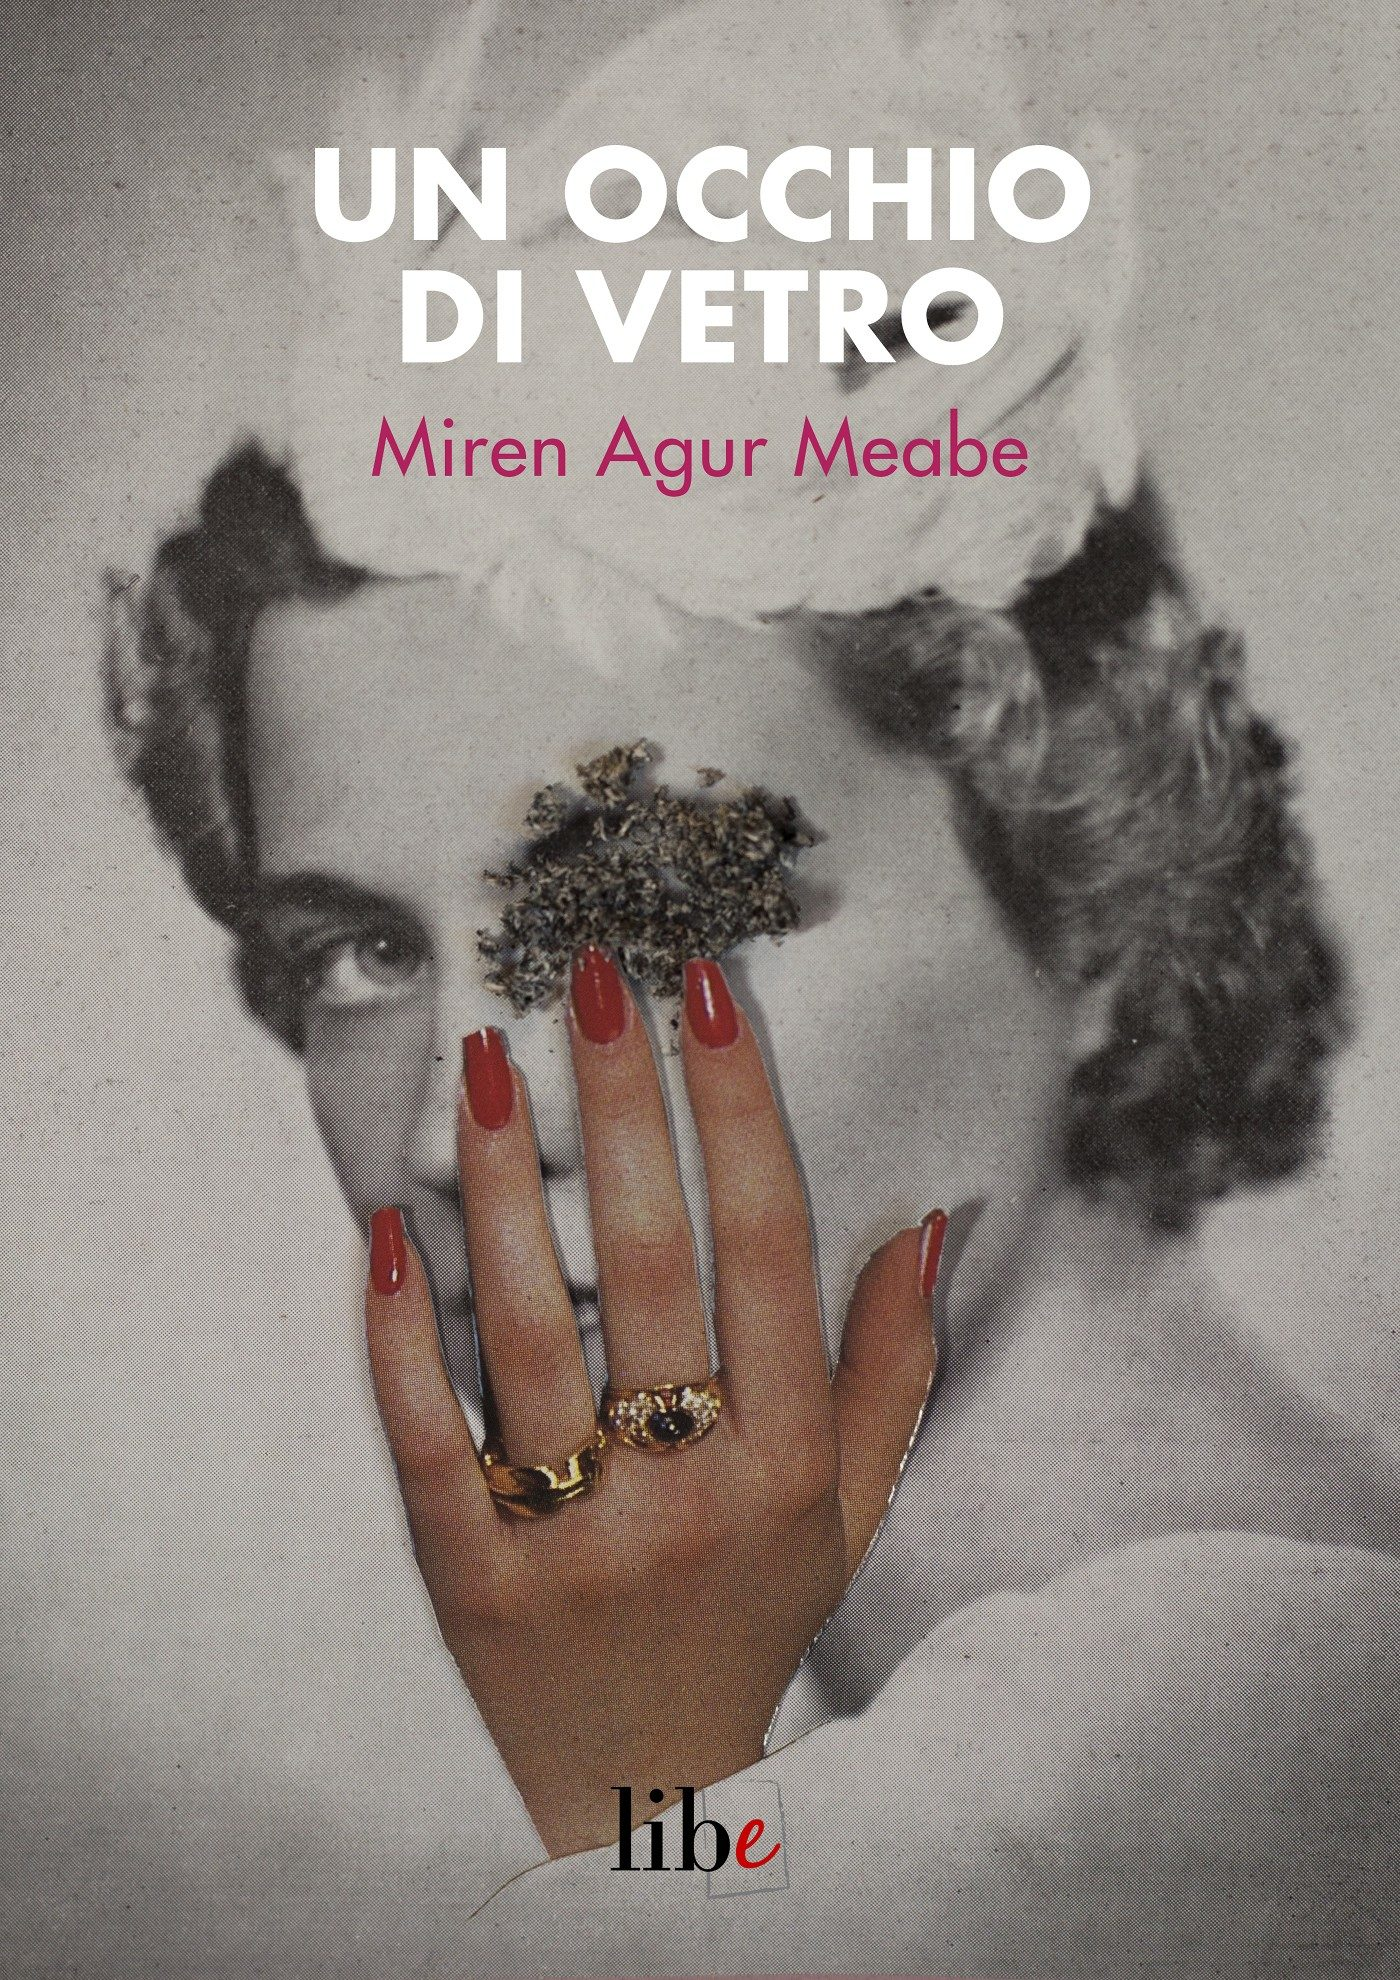
\includegraphics[width=0.7\textwidth]{inc/images/cover.jpg}
  %     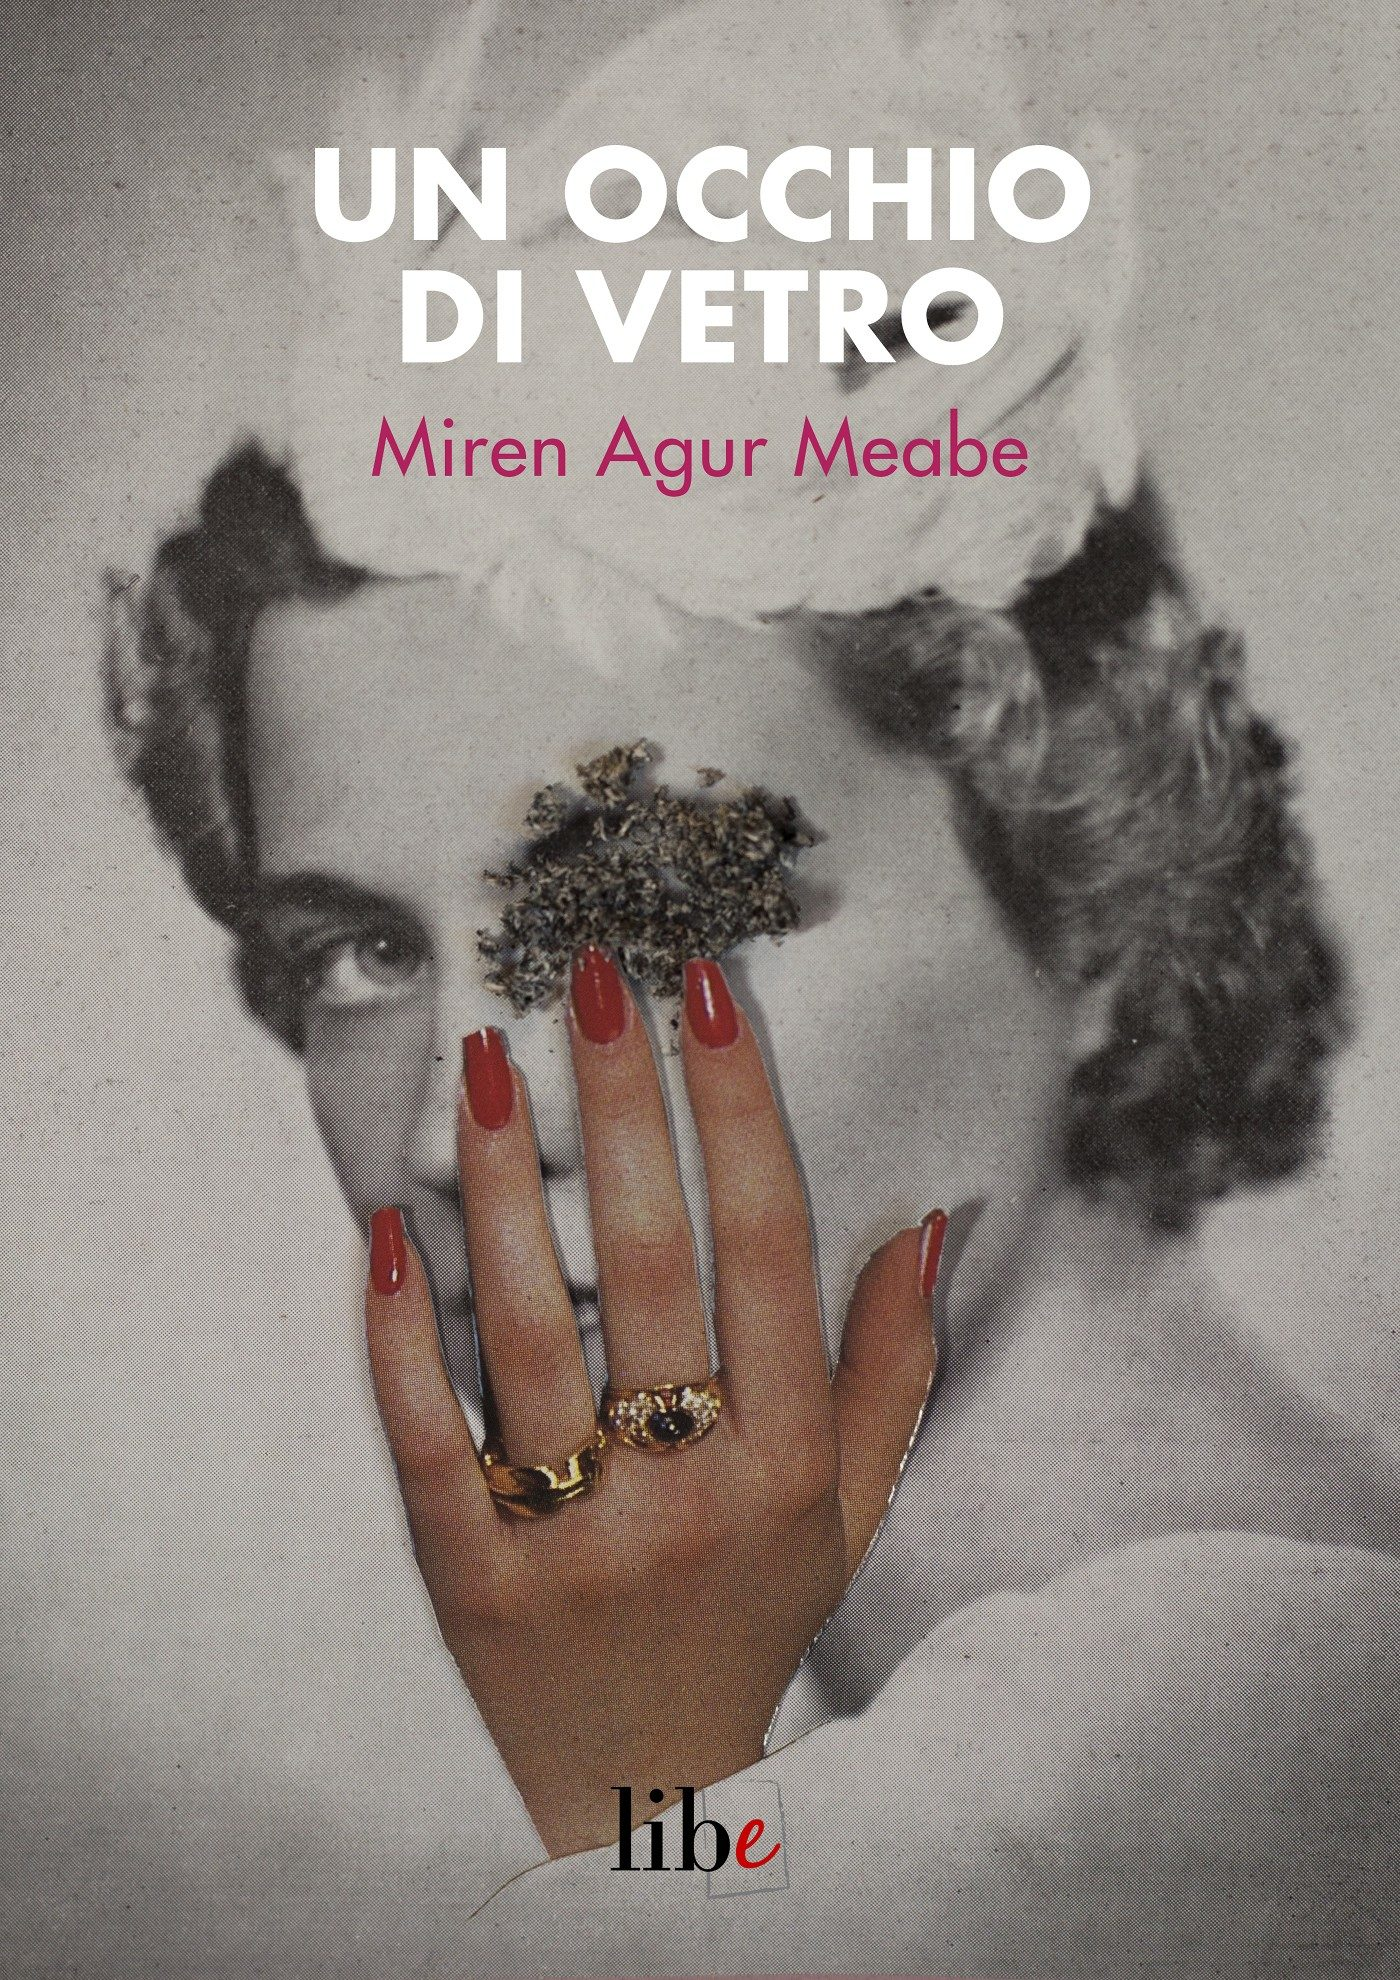
\includegraphics[width=\paperwidth]{inc/images/cover.jpg}
  %   \end{center}
  % \vspace*{\fill}
  %
  % \newpage\null\thispagestyle{empty}\newpage

  $for(include-before)$
  $include-before$

  $endfor$

  \frontmatter

  % \thispagestyle{empty}
  \begin{figure}[p]
      \vspace*{-12mm}
      \hspace*{-12.5mm}
      \makebox[\paperwidth]{
            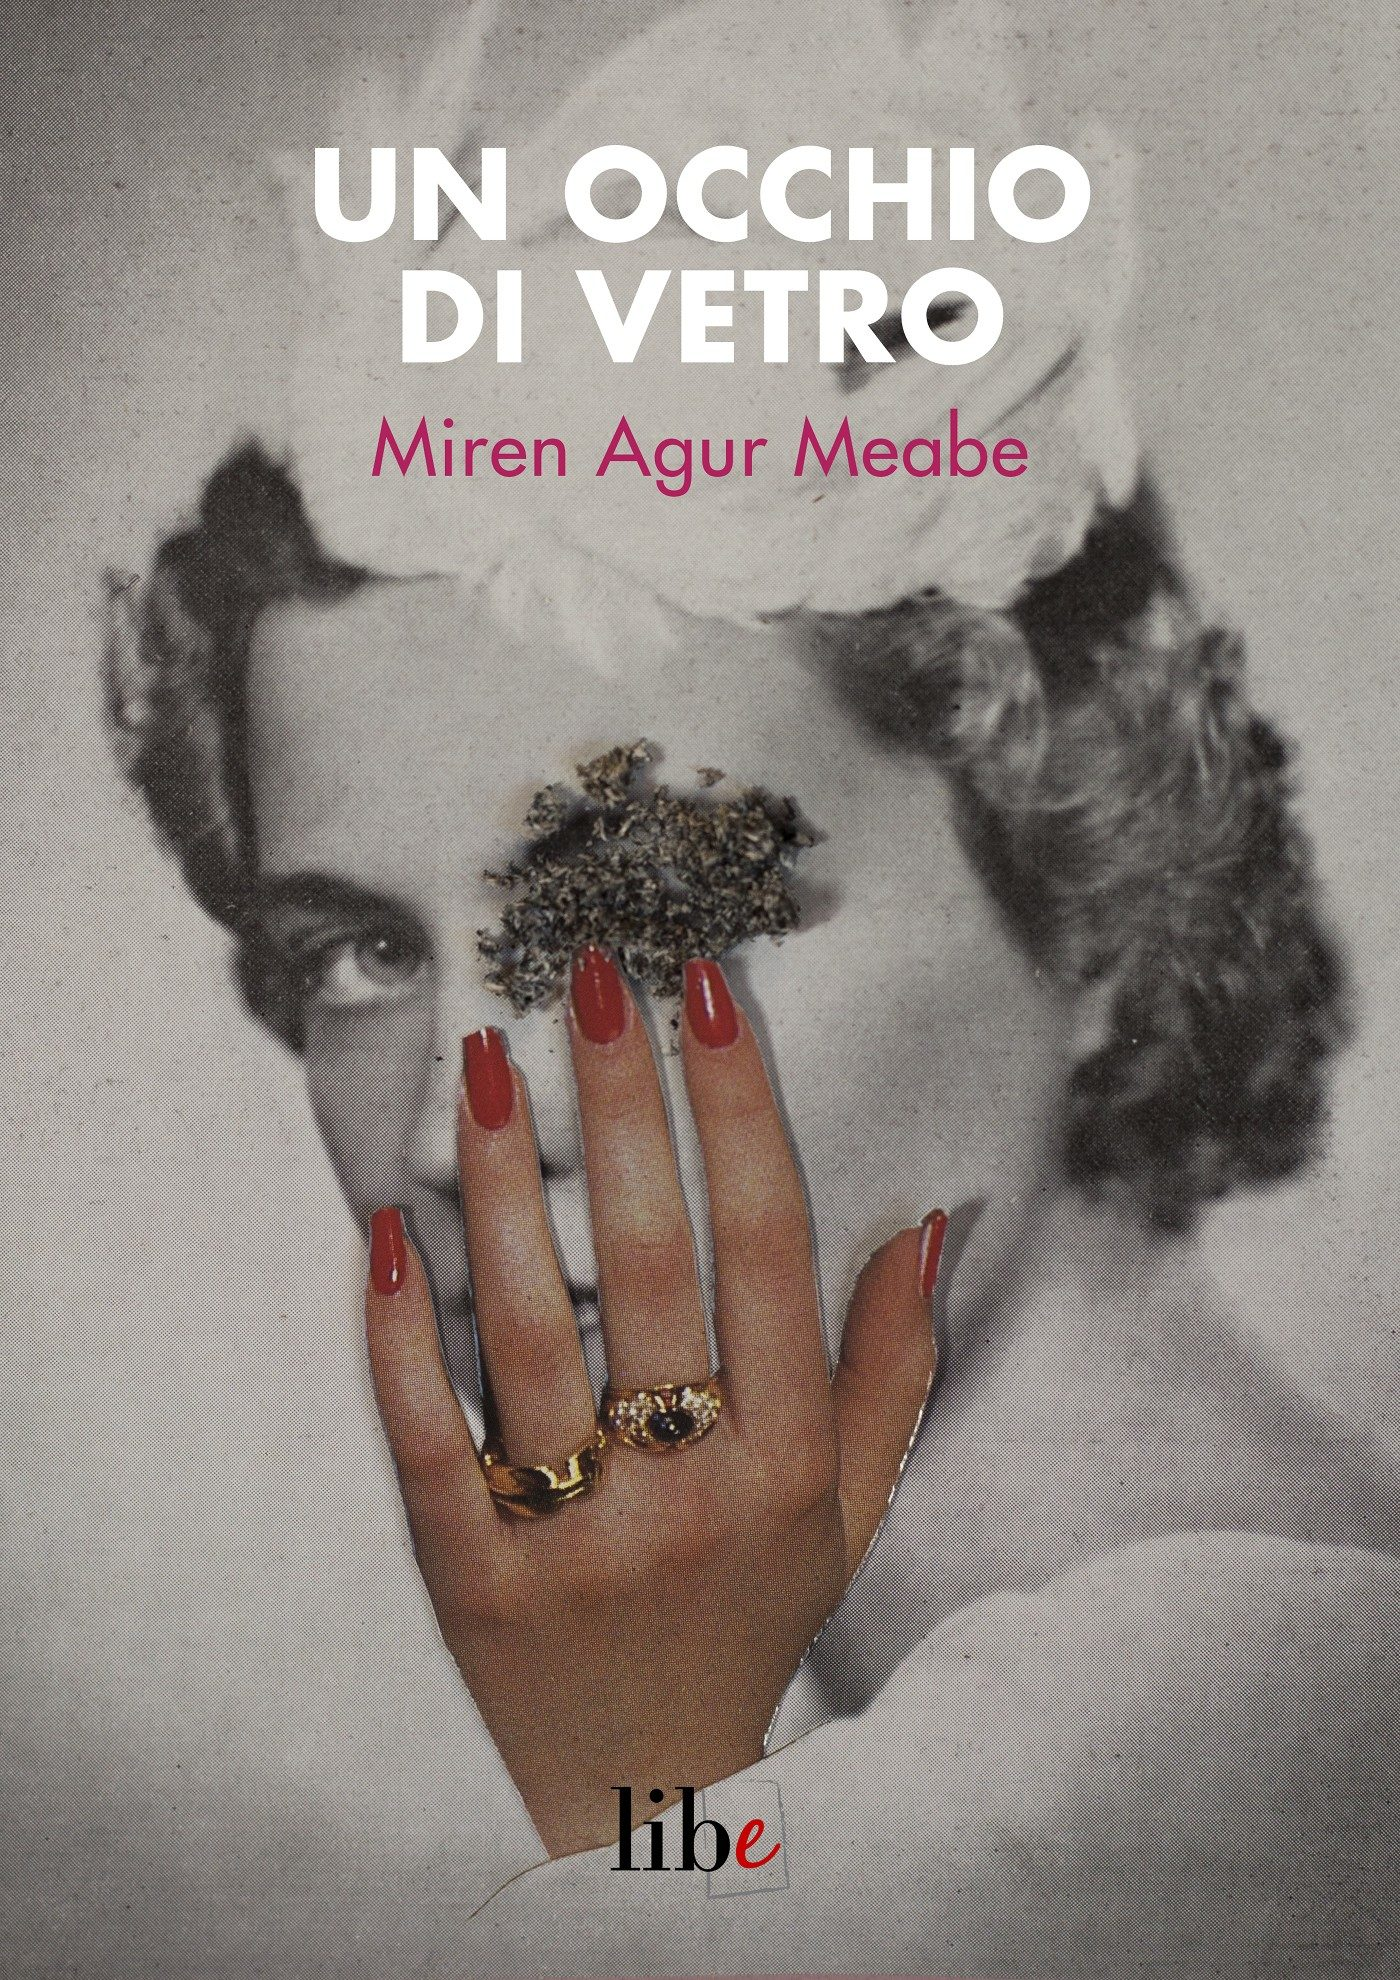
\includegraphics[width=1\paperwidth]{inc/images/cover.jpg}
      }
  \end{figure}

  $if(title)$
    \maketitle
  $endif$

  $if(abstract)$
    \begin{abstract}
  $abstract$
    \end{abstract}
  $endif$


  % \setcounter{page}{0}

  % Book contents
  \mainmatter{}

  $body$

  \backmatter{}

  $if(toc)$
  {
  $if(colorlinks)$
    \hypersetup{linkcolor=$if(toccolor)$$toccolor$$else$black$endif$}
  $endif$
    \setcounter{tocdepth}{$toc-depth$}
    \tableofcontents
  }
  $endif$

  $if(lot)$
    \listoftables
  $endif$

  $if(lof)$
    \listoffigures
  $endif$


  $for(include-after)$
  $include-after$

  $endfor$
\end{document}
